\documentclass[12pt,a4paper]{article}
\usepackage[brazilian]{babel} %Traduz o documento para o portugues do brasil
\usepackage[utf8]{inputenc} %Reconhece acentuação
\usepackage{lipsum} %Gera texto aleatório
\usepackage{graphicx}


\begin{document}
%\newcommand{\DIR}{DIR = /}
	
{\LARGE Estatística - 1}
\newline
\newline
\textbf{{\large Amostragem}}

\textbf{\textit{\\Conceitos}} 

\textbf{\textit{\\População}}: Alvo do estudo.
\textbf{\textit{\\\\Censo}}: Pesquisa com toda a população, pode ser caro ou impossível inferir sobre toda a população.
\textbf{\textit{\\\\Enviesamento}}: Você subestima ou superestima o parâmetro da população. 
\textit{causas}: Pesquisa de pessoas próximas ou de fácil acesso, pesquisas pela internet, sem uso de mecanismo de seleção aleatório.

\textbf{\textit{\\Amostra}} - Parte de uma população (Subconjunto da população), selecionada usando alguma técnica que de chances iguais a todos os elementos da população de serem selecionados. 
\\\\Uma amostra feita corretamente deve representar as mesmas características da população de onde foi retirada.
\\\\Se ela não representa a população, dizemos que ela é enviesada.
\textbf{\\\\"Custo" da Amostra}
\\Margem de erro e nível de confiança.
\\Variação: amostrar diferentes podem apresentar resultados diferentes.
\\podemos "medir" a variação esperada.

\newpage

\textbf{\textit{\\Principais tipos de amostras}} 

\textbf{\textit{\\Aleatória simples - }}
Um determinado número de elementos é retirado da população de forma aleatória.
Todos os elementos da população alvo do processo de amostragem, devem ter as mesmas chances 
de serem selecionado para fazer parte da amostra.


{\centering 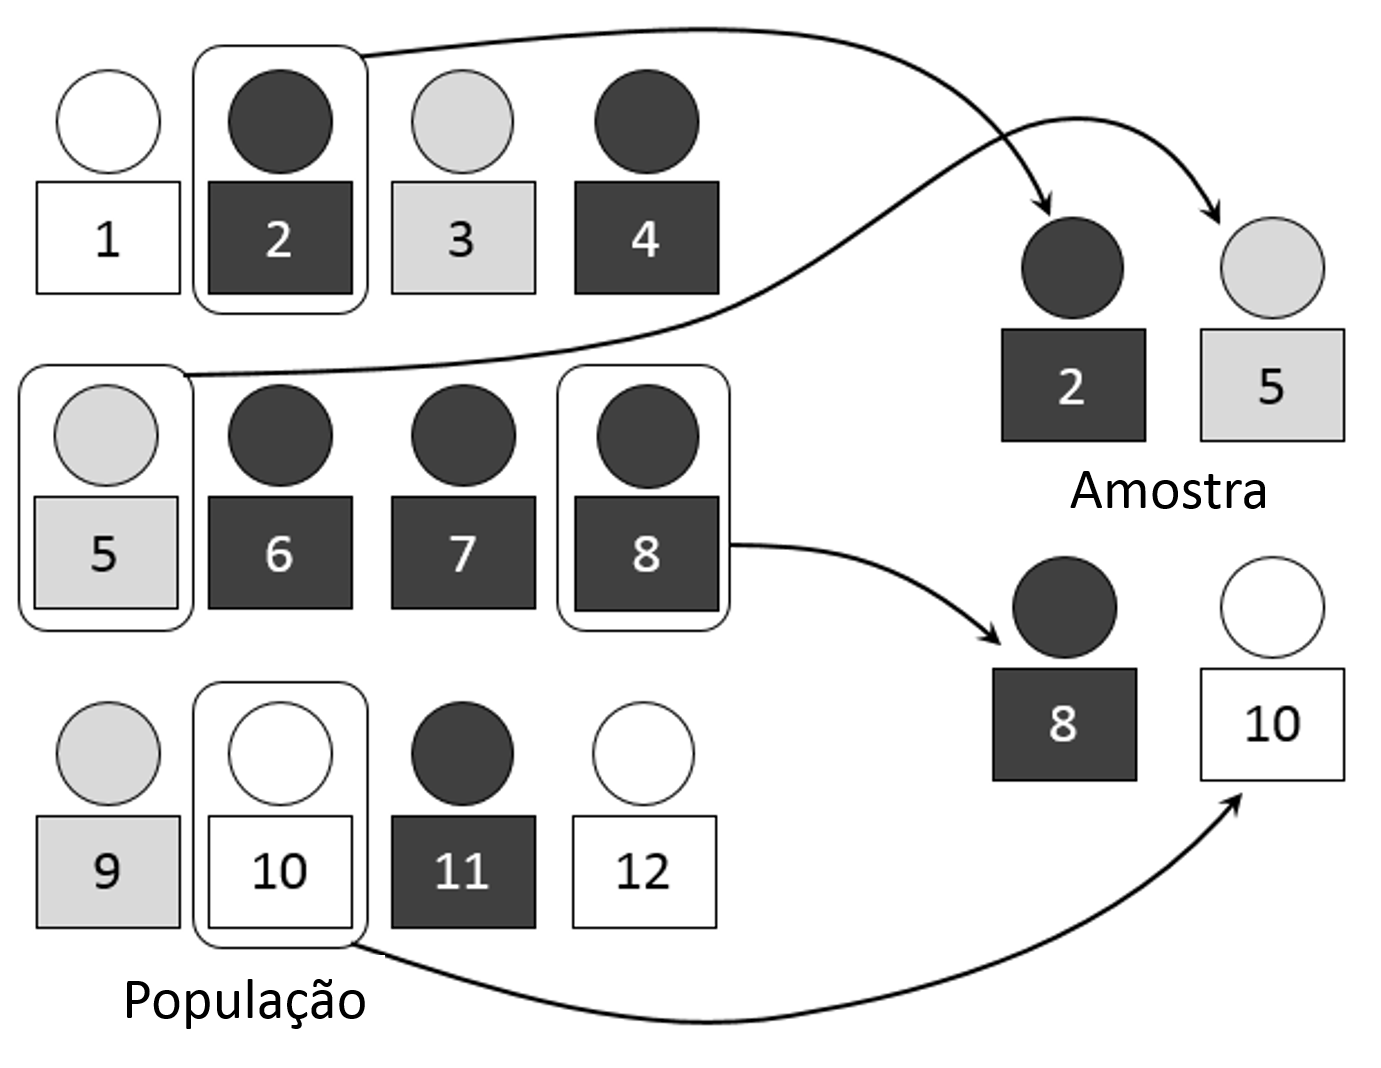
\includegraphics[scale=0.17]{Amostragem/AleatoriaSimples.png} \par}

Há duas formas de trabalhar com amostra aleatória simples, com reposição e sem reposição. 

\textit{Com reposição:}
Quer dizer que uma vez que o elemento da população é selecionado, ele volta a fazer parte da população 
e ele passa a ter as mesmas chances de ser selecionado novamente, exemplo(Exame de dopping em atletas das olimpíadas). 

{\centering 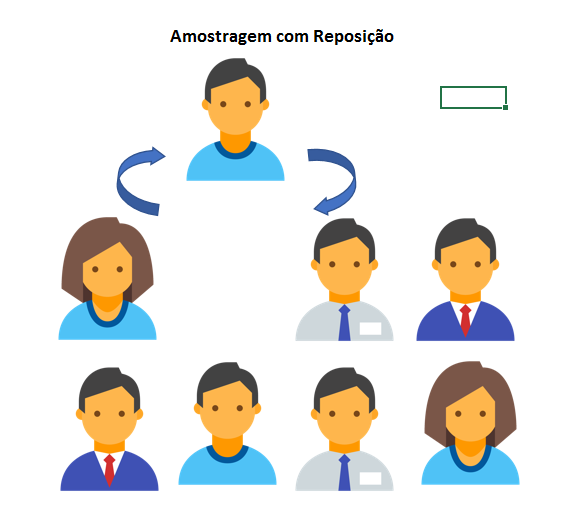
\includegraphics[scale=0.45]{Amostragem/amostragemComReposicao.png} \par}

\newpage

\textit{Sem reposição:}
Uma vez que o elemento da população é selecionado, ele não faz mas parte da população e não tem mais chance ser selecionado novamente, exemplo(Pesquisa de intensão de votos). 

{\centering 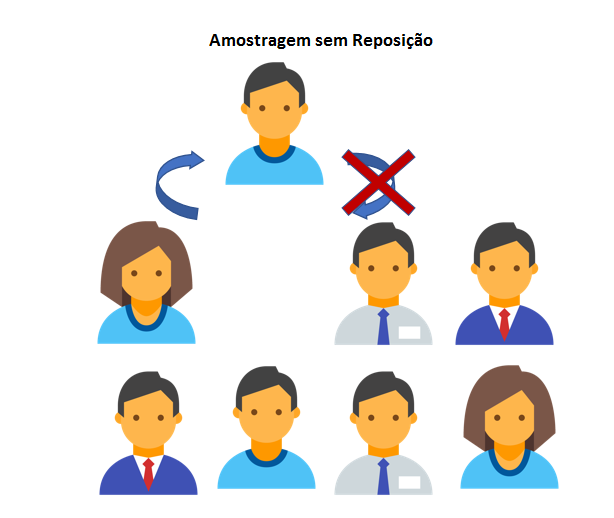
\includegraphics[scale=0.45]{Amostragem/amostragemSemReposicao.png} \par}

\textbf{\textit{\\Estratificada -}}
As vezes as populações estão divididas nos chamados estratos, características comuns que os elementos tem, podem ser relacionados a raça, escolaridade ou religião.

{\centering 
\includegraphics[scale=0.45]{Amostragem/amostragemEstratificada.jpg} \par}

\textbf{\textit{\\Sistemática -}}
Neste tipo de amostragem, é escolhido um elemento aleatório, e a partir daí, a cada N elementos um novo membro é escolhido.

{\centering 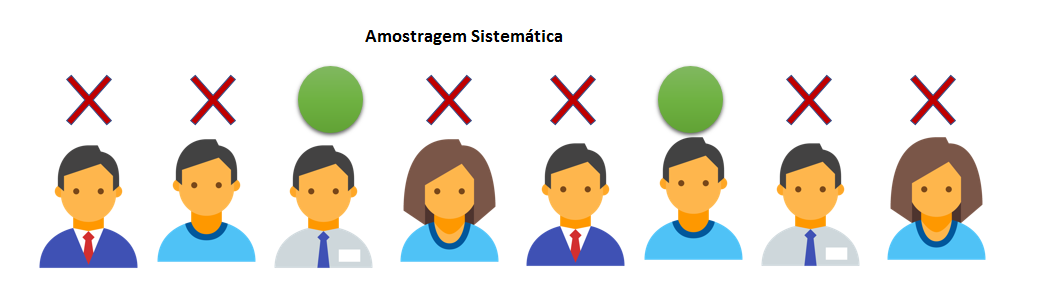
\includegraphics[scale=0.45]{Amostragem/amostragemSistematica.png} \par}

\newpage

\textbf{\textit{\\Por Unidade Monetária -}}
Neste tipo de amostra é informada uma coluna de ordenação, e uma coluna numérica que sera utilizada 
para gerar os cálculos para produzir a amostra.

{\centering 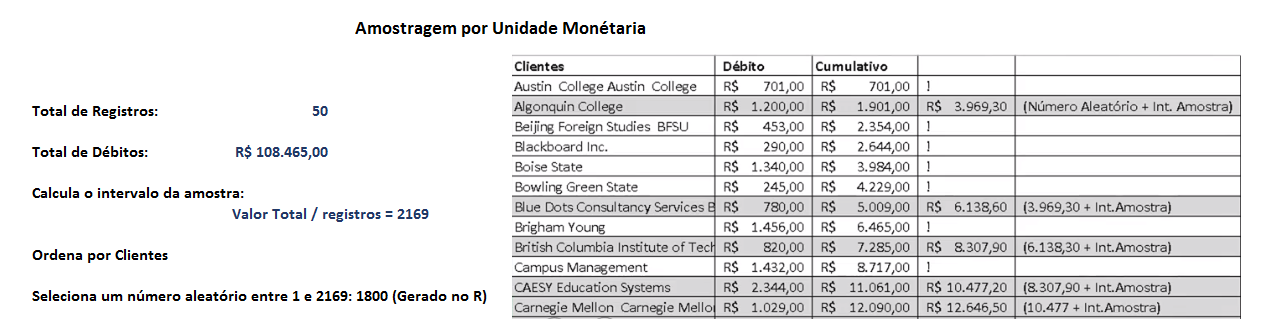
\includegraphics[scale=0.45]{Amostragem/amostragemPorUnidadeMonetaria.png} \par}

	
\end{document}